\documentclass[12pt]{article}

\usepackage{sbc-template}


\usepackage{graphicx,url,multirow,multicol}
\usepackage{amssymb,amsmath,latexsym,mathabx,wasysym,stmaryrd}
\usepackage[brazil]{babel}
\usepackage[utf8]{inputenc} 
\usepackage{colortbl}

\sloppy

%\title{Inferência de Desempenho: Uma Nova Abordagem para Planejar a Capacidade de Aplicações na Nuvem}
\title{Inferência de Desempenho: Uma Nova Abordagem para o Planejamento da Capacidade de Aplicações na Nuvem}
\author{Marcelo Gonçalves, Matheus Cunha, Américo Sampaio, Nabor C. Mendonça}

\address{Programa de Pós-Graduação em Informática Aplicada (PPGIA)\\
Universidade de Fortaleza (UNIFOR)\\
Av. Washington Soares, 1321, Edson Queiroz, CEP 60811-905 Fortaleza, CE
\email{\{marcelocg,mathcunha\}@gmail.com,\{americo.sampaio,nabor\}@unifor.br}
}

\begin{document} 

\maketitle

\begin{resumo} 

%Um dos principais desafios enfrentados pelos usuários de nuvens que oferecem infraestrutura- como-serviço (IaaS) é planejar adequadamente a capacidade dos recursos da nuvem necessários às suas aplicações. 

Este trabalho propõe uma nova abordagem para apoiar o planejamento da capacidade de aplicações em nuvens que oferecem infraestrutura-como-serviço (IaaS). A abordagem proposta tem como premissa a existência de uma relação de capacidade entre diferentes configurações de recursos de um dado provedor de nuvem IaaS, com a qual é possível prever (ou ``inferir''), com alta precisão, o desempenho esperado de uma aplicação para certas configurações de recursos e cargas de trabalho, tendo com base o desempenho da aplicação observado para outras configurações de recursos e cargas de trabalho neste mesmo provedor. Resultados empíricos preliminares, obtidos a partir da avaliação do desempenho de uma popular aplicação de \emph{blogging} (WordPress) em um provedor de nuvem público (Amazon), mostram que a nova abordagem consegue reduzir significativamente (acima de 80\%) o número total de cenários de implantação da aplicação que precisam de fato ser avaliados na nuvem.

\end{resumo}

\begin{abstract}

%One of the main challenges faced by users of infrastructure-as-a-service (IaaS)  clouds is to adequately plan the cloud resources required to the meet their applications' needs. 

This work proposes a novel approach to support application capacity planning in infrastructure-as-a-service (IaaS) clouds. The proposed approach relies on the assumption that there exists a capacity relation between different resource configurations offered by a given IaaS cloud provider, enabling one to predict (or ``infer''), with high accuracy, an application's expected performance for certain resource configurations and workloads, based upon its observed performance for other resource configurations and workloads in that same provider. Preliminary empirical results, obtained from evaluating the performance of a well-known blogging application (WordPress) in a public cloud provider (Amazon), show that the proposed approach can significantly reduce (over 80\%) the total number of application deployment scenarios that need to be effectively tested in the cloud.

\end{abstract}

\section{Introdução}\label{sec:introducao}

%A computação em nuvem é um paradigma computacional que está transformando a forma de desenvolver e gerenciar aplicações e serviços de Tecnologia da Informação \cite{Murugesan2014}. Diversas organizações passaram a adotar este paradigma atraídas pelo seu modelo de negócios onde recursos computacionais (ex.: computação, armazenamento e transferência de dados) podem ser consumidos, sob-demanda, como um serviço e pagos de acordo com o consumo efetuado. 

Um dos principais desafios enfrentados pelos usuários de nuvens que oferecem infraestrutura-como-serviço (IaaS) é a planejar adequadamente a capacidade dos recursos da nuvem necessários para atender as demandas específicas de suas aplicações \cite{Menasce2009}.  Parte desse desafio envolve tentar descobrir a melhor maneira de implantar a aplicação na nuvem, considerando os vários tipos de recursos (em particular, máquinas virtuais) oferecidos pelo provedor, sob a perspectiva de diferentes requisitos e critérios de qualidade \cite{GoncalvesJunior2015}.  

Em geral, provedores de nuvens IaaS cobram seus usuários em função do tempo de utilização dos recursos solicitados, cujos preços variam conforme a capacidade (normalmente medida por características técnicas como quantidade de núcleos de processamento, tamanho de memória e espaço de armazenamento) de cada recurso. Dessa forma, para calcular o custo de operação de uma aplicação na nuvem, é preciso estimar ou medir como a aplicação responderá a diferentes níveis de demanda, em termos de indicadores de desempenho como tempo de resposta ou vazão, quando executada sob diferentes configurações e perfis de máquinas virtuais. Somem-se a isso as inúmeras possibilidades de implantação da aplicação considerando tanto estratégias de escalabilidade vertical (variando-se a quantidade de recursos de cada máquina) quanto horizontal (variando-se a quantidade de máquinas em uma ou mais camadas da aplicação, como dados, apresentação e negócio), chega-se a um conjunto bastante amplo de cenários de implantação a serem investigados. Assim, torna-se fundamental identificar, dentre as possíveis configurações de máquinas virtuais ofertadas por um ou mais provedores de nuvem, aquelas de menor custo capazes de executar a aplicação mantendo-se níveis satisfatórios para os indicadores de desempenho.

Outro desafio ao planejamento de capacidade decorre da constatação de que configurações formadas por recursos com perfis similares, ainda que do mesmo provedor, podem responder de maneira diferente quando submetidas a um mesmo nível de carga de trabalho, a depender do momento em que sejam utilizadas \cite{cunha2011investigating, iosup2011performance, jayasinghe2011variations}. Independente do motivo que leve a esse comportamento de certa forma imprevisível, é preciso levar em conta nos testes de avaliação de desempenho essa variabilidade, o que pode pode ser alcançado através da repetição dos cenários de teste em horários e dias diferentes.

Um grande problema começa a se desenhar ao seguir essa abordagem: a fase de avaliação da aplicação pode atingir patamares elevados de tempo e custo, em razão das necessidades de variação da demanda, da arquitetura de implantação e das configurações de recursos utilizadas para avaliar cada arquitetura implantada \cite{silva2013cloudbench}. 
Ainda que certos provedores IaaS ofereçam descontos ou pacotes de horas grátis para novos clientes, em geral esses incentivos são suficientes para custear apenas algumas semanas de utilização de umas poucas máquinas virtuais de pequeno porte, muito provavelmente incapazes de suportar a carga de uma aplicação real em produção. Assim, executar 
uma aplicação real, tipicamente implantada em arquitetura de várias camadas, em máquinas virtuais de tamanho considerável e por longos períodos de tempo apenas para estudar o seu comportamento, pode se traduzir em um custo alto que dificulte ou até mesmo inviabilize o próprio projeto de migração dessa aplicação para a nuvem. 

Vários trabalhos já foram propostos com o intuito de apoiar o planejamento da capacidade de aplicações em nuvens IaaS (e.g., \cite{cloudharmony, malkowski2010cloudxplor, fittkau2012cdosim, li2011cloudprophet, jayasinghe2012, silva2013cloudbench, cunha2013b, jung2013cloudadvisor, scheuner2014cloud}). Em linhas gerais, esses trabalhos seguem duas abordagens distintas quanto à estratégia de avaliação do desempenho da aplicação: a \emph{abordagem preditiva}, cujo objetivo é tentar prever o desempenho esperado da aplicação para determinadas configurações de recursos e determinados níveis\l de carga, sem necessariamente ter que implantá-la na nuvem  \cite{cloudharmony, malkowski2010cloudxplor, fittkau2012cdosim, li2011cloudprophet, jung2013cloudadvisor}; e a \emph{abordagem empírica}, cujo objetivo é medir o desempenho real da aplicação através de sua efetiva implantação na nuvem e da realização de testes de carga \cite{jayasinghe2012, silva2013cloudbench, cunha2013b, scheuner2014cloud}. As técnicas de predição de desempenho adotadas na abordagem preditiva variam conforme o trabalho, sendo as mais comuns o uso de simuladores \cite{fittkau2012cdosim} e a analogia com resultados previamente obtidos através da utilização de \emph{benchmarks} \cite{cloudharmony, malkowski2010cloudxplor}. Apesar do baixo custo oferecido aos usuários, que não precisam pagar por recursos de nuvem durante a fase de avaliação, trabalhos da abordagem preditiva têm como maior limitação uma ainda baixa precisão na sua  capacidade de prever o desempenho da aplicação alvo. Isto se deve principalmente a diferenças conceituais entre o ambiente da nuvem real e os modelos de simulação \cite{fittkau2012cdosim}, ou à ausência de \emph{benchmarks} com comportamento e perfis de carga de trabalho similares aos da aplicação alvo. Já os trabalhos que utilizam a abordagem empírica, por executarem a aplicação no próprio ambiente de nuvem, conseguem obter resultados significativamente mais precisos no que diz respeito à seleção das melhores configurações de recursos para cargas de trabalho específicas. No entanto, uma limitação importante desses trabalhos é a necessidade de se testar exaustivamente uma grande quantidade de configurações de recursos e cargas de trabalho, implicando em altos custos durante a fase de avaliação.

Visando combinar as vantagens das abordagens preditiva e empírica, este trabalho propõe uma nova maneira de apoiar os usuários de nuvens IaaS a identificarem as melhores (i.e., mais baratas) configurações de recursos capazes de satisfazer as demandas específicas de suas aplicações. A nova abordagem tem como premissa a existência de uma relação de capacidade entre diferentes configurações de recursos oferecidas por um dado provedor de nuvem, com a qual é possível prever (ou ``inferir''), com alta precisão, o desempenho esperado da aplicação para determinadas configurações de recursos. A predição ou inferência é realizada com base no desempenho observado da aplicação para outras configurações de recursos e cargas de trabalho no mesmo provedor. Por exemplo, se a aplicação atendeu satisfatoriamente a demanda para uma configuração de recursos de determinada capacidade sob um determinada carga de trabalho, é muito provável que ela também vá atendê-la para outras configurações de maior capacidade sob a mesma carga de trabalho. Analogamente, se a aplicação não atendeu a demanda para uma determinada configuração de recursos sob uma determinada carga de trabalho, muito provavelmente ela também não irá atendê-la para a mesma configuração sob cargas de trabalho maiores. Através do processo de inferência, a abordagem permite avaliar uma ampla variedade de cenários de implantação da aplicação, sendo que apenas uma pequena parte desses cenários precisa de fato ser implantada e executada na nuvem. Dessa forma, a abordagem consegue obter o melhor das duas abordagens previamente citadas, produzindo resultados de alta precisão (característicos da abordagem empírica) mas com significativa redução de custo (característica da abordagem preditiva).

A próxima seção define alguns conceitos úteis para o entendimento do trabalho. A seção~\ref{sec:process} descreve o novo processo de avaliação de capacidade por inferência de desempenho, destacando suas atividades e sua implementação. A seção~\ref{sec:experiments} reporta a metodologia utilizada e os resultados obtidos em uma avaliação experimental do processo. A seção~\ref{sec:related-work} compara o novo processo com outros trabalhos relacionados. Por fim, a seção~\ref{sec:conclusion} oferece algumas conclusões e sugestões para trabalhos futuros.

\section{Fundamentos e Terminologia}\label{sec:background}

Antes de apresentar o novo processo de avaliação de capacidade, é necessário definirmos alguns conceitos úteis para o seu entendimento. Esses conceitos também servirão para estabelecer a terminologia utilizada na descrição do processo bem como de sua avaliação.

%\vspace{-2.5\parskip}\paragraph{\em <term to be defined>}
%\smallskip\noindent\textbf{\em <term to be defined>}\enskip

\begin{description}

\smallskip
\item[\em Aplicação sob teste] 
Um sistema computacional, possivelmente implementado em uma arquitetura multicamadas, para o qual se deseja observar o comportamento em um ambiente de computação em nuvem e ao qual estão associadas uma ou mais {\em métricas de 
desempenho}.

\item[\em Métrica de desempenho] 
Uma característica ou comportamento mensurável de forma automatizada e comparável a um {\em valor de referência}, capaz de indicar o grau de sucesso de uma execução da aplicação sob teste. É dependente do domínio da aplicação. Ex.: tempo de resposta, quadros por segundo, bits por segundo, etc.

\item[\em Valor de referência (SLA)] 
Um valor predefinido como minimamente aceitável  para uma métrica de desempenho após uma execução da aplicação sob teste. Este valor, também referenciado neste trabalho como SLA (\emph{Service Level Agreement}), serve como base de comparação para que se classifique a aplicação como capaz de ser executada em uma determinada {\em configuração} de máquinas virtuais e sob uma determinada {\em carga de trabalho}.

\item[\em Provedor]
Uma empresa que fornece recursos computacionais como serviço cobrado financeiramente por fração de tempo de utilização. Neste trabalho, o foco será em provedores que disponibilizam recursos de infraestrutura, notadamente {\em máquinas virtuais}.

\item[\em Tipos de máquinas virtuais]
Classificam as máquinas virtuais fornecidas por um provedor conforme suas características técnicas, como capacidade de processamento, quantidade de memória, e quantidade de espaço em disco, permitindo que o provedor mantenha uma linha de produtos discreta e finita.

\item[\em Categoria]
Os tipos de máquinas virtuais de um provedor podem ser agrupados em {\em categorias}, conforme suas características técnicas, plataforma e/ou arquitetura de hardware e a natureza do uso a que se destinam. Dentro de uma mesma categoria, os tipos de máquinas virtuais variam apenas na quantidade de cada um dos recursos especificados para a categoria e no preço cobrado pelo uso das máquinas virtuais. Ex.: categorias que priorizam consumo de memória, acesso a disco, processamento gráfico, etc. 

\item[\em Configuração]
Um conjunto de máquinas virtuais de um mesmo tipo e, portanto, de uma mesma categoria. {\em Configurações} são usadas para implantar uma ou mais camadas arquiteturais (ex.: apresentação, negócio, persistência, etc.) da aplicação sob teste.

\item[\em Espaço de implantação]
Denota um conjunto limitado de configurações de máquina virtuais nas quais a aplicação sob teste será implantada e executada durante uma sessão de avaliação. 

\item[\em Carga de trabalho]
Representa o tamanho da demanda que será imposta à aplicação sob teste em uma execução. Sua unidade de medida é dependente do domínio da aplicação. Ex.: tamanho dos arquivos de entrada para uma aplicação de compactação de arquivos, quantidade de usuários concorrentes para uma aplicação web, etc.

\item[\em Cenário de execução]
Corresponde à execução da aplicação sob teste utilizando uma determinada configuração de máquinas virtuais e submetida a uma determinada carga de trabalho. O resultado de um {\em cenário de execução} fornece indicadores que permitirão avaliar se a aplicação atingiu o valor de referência (SLA) esperado para uma determinada métrica de desempenho naquele cenário.

\end{description}

\section{Processo de Avaliação de Capacidade por Inferência de Desempenho}\label{sec:process}

\subsection{Visão Geral do Processo}

O processo de avaliação de capacidade proposto neste trabalho (ver Figura~\ref{fig:fig_processo_alto_nivel}) prevê um conjunto de dados de entrada, uma ou mais execuções da aplicação sob teste no ambiente de nuvem almejado para 
hospedá-la, e a análise do desempenho obtido pela aplicação a partir dos resultados de suas execuções. Com base nos dados de desempenho, o processo passa por diversos pontos de decisão que podem levar a novas execuções da aplicação utilizando diferentes configurações de máquinas virtuais e sob diferentes níveis de carga. Ao final do processo, é fornecida como saída uma lista de configurações, ordenadas por preço, capazes de obter o desempenho esperado da aplicação para cada nível de carga avaliado.

\begin{figure}[t]
  \begin{center}
    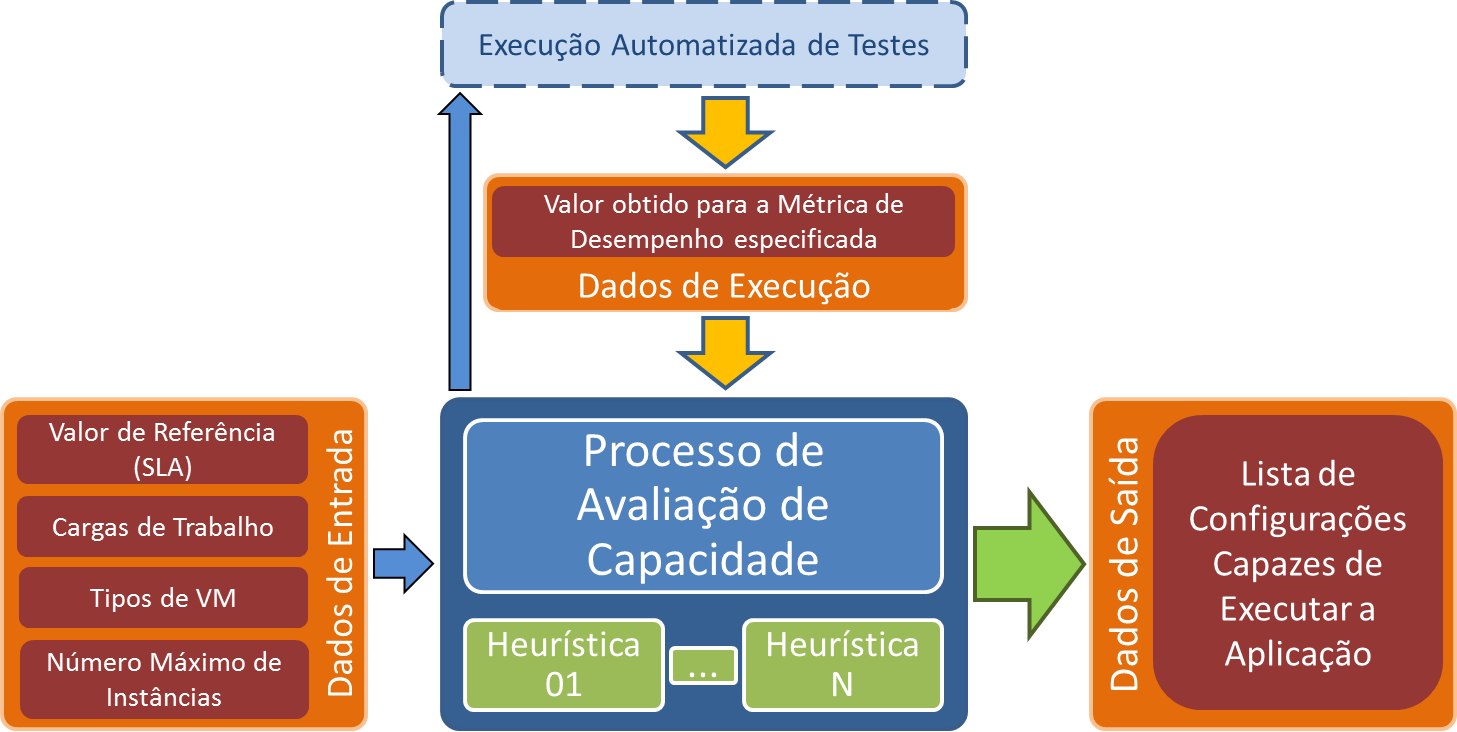
\includegraphics[scale=0.45]{img/processoAltoNivel}
  \end{center}
  \caption{\label{fig:fig_processo_alto_nivel}Visão geral do Processo de  Avaliação de Capacidade.}
\end{figure}

O restante desta seção aborda em detalhes todas as etapas do processo proposto, explicando quais são os dados recebidos como entrada, as diferentes atividades executadas e as decisões a serem tomadas para que o processo possa determinar as configurações que atendem os requisitos de desempenho e carga de trabalho da aplicação.

\subsubsection{Dados de Entrada}

O principal dado de entrada esperado pelo processo é o valor de referência (SLA), o qual será usado para determinar 
se a aplicação atingiu os requisitos mínimos de desempenho exigidos em cada cenário de execução. Além do SLA, o processo precisa também conhecer quais são as cargas de trabalho sob as quais o desempenho da aplicação deverá ser avaliado. Outro dado importante que deve ser passado como entrada para o processo é o espaço de implantação da aplicação. Para isso, o processo deve ser alimentado com dois parâmetros: (i) uma lista de tipos de máquinas virtuais fornecidos pelo provedor no qual deseja-se hospedar a aplicação; e (ii) a quantidade máxima de máquinas virtuais de cada tipo que irá compor cada configuração a ser avaliada. Para dar um exemplo, suponhamos que o processo recebeu como entrada uma lista com dois tipos de máquinas virtuais, $T_{1}$ e $T_{2}$, e o valor 

Porém,
nem todas as Cargas de Trabalho serão impostas de fato à Aplicação. Isso vai 
depender do conjunto de decisões tomadas pelo processo com base na comparação do 
resultado obtido pela Aplicação com o SLA. Ainda assim, graças à sua característica 
de inferência de desempenho, o processo mostra resultados para todas as Cargas de 
Trabalhado informadas como parâmetro de entrada.

Para que o desempenho da Aplicação seja avaliado, é preciso que o processo conheça 
quais são as Configurações disponibilizadas no Provedor de nuvem para esse fim. 
Para isso, o processo deve ser alimentado com uma lista de Tipos de Máquinas Virtuais 
que serão utilizadas na execução da Aplicação, bem como a quantidade máxima de 
instâncias usadas para compor cada Configuração. Através desses dados o processo
passa a conhecer então o Espaço de Implantação disponível para os testes de 
desempenho, composto por uma lista de Configurações geradas a partir da lista de
Tipos de Máquinas Virtuais disponíveis e do número máximo de instâncias.

\subsubsection{Atividades Customizáveis}
O processo de avaliação de capacidade proposto é um processo extensível, do qual
fazem parte atividades customizáveis para as quais são delegadas funções de
cunho mais específico, como a comunicação com o Provedor de nuvem e a Aplicação sob Teste
para fins de orquestração do teste de desempenho, e também funções para as quais
é desejado um certo grau de flexibilidade a fim de tornar o processo mais adaptável,
como a escolha das Cargas de Trabalho e Configurações que serão usadas na execução
da Aplicação.

\paragraph{Execução dos Testes de Desempenho}
Todas as atividades ligadas à rotina de execução da Aplicação, desde sua implantação,
passando pela criação e configuração das máquinas virtuais no ambiente do Provedor 
de nuvem, bem como pelo controle de inicialização e finalização dessas instâncias, 
serviços subjacentes como bancos de dados e filas, e a própria parametrização da 
execução e parada da Aplicação em si não fazem parte do escopo do processo. Este,
por sua vez, presume que os dados de resultado para cada execução estarão disponíveis
quando necessários. A maneira como esses dados serão de fato obtidos é
encapsulada pela implementação concreta desta atividade do processo.

%dependente da implementação concreta do processo e é irrelevante do ponto de
%vista do seu funcionamento.  

Portanto, o processo prevê a customização da atividade de Execução dos Testes,
que será responsável pelas ações necessárias à execução da Aplicação sob Teste no ambiente
alvo. A atividade customizada deverá conhecer os detalhes inerentes à comunicação com 
o Provedor e com a Aplicação sob Teste e, assim, ser capaz de ordenar a sua execução e 
coletar como resposta os dados de desempenho esperados pelo processo. Esse é um dos 
pontos de extensibilidade oferecidos pelo processo, cuja implementação concreta está 
fora do escopo deste trabalho. Vale destacar que o foco do processo proposto não está na automação de execução de testes de qualquer natureza, mas na análise dos dados resultantes dessa execução.

\paragraph{Estratégias e Heurísticas}
\label{subsubsec:heuristicas}
De modo análogo à abordagem adotada em relação às atividades de execução dos
testes, as operações de seleção da Configuração sobre as quais a Aplicação
sob Teste será executada, bem como a seleção das Cargas de Trabalho a que ela 
será submetida durante sua execução, não são executadas diretamente pelo processo.
Nesse caso, são delegadas a uma atividade customizada que chamamos de Estratégia de 
Avaliação ou, simplesmente, Estratégia. Seu objetivo é permitir a aplicação de 
diferentes métodos para a escolha da melhor Configuração e/ou Carga de Trabalho 
mais adequada aos objetivos da avaliação de capacidade em curso e também ao perfil 
da Aplicação.

Como veremos na seção~\ref{sec:funcionamento_processo}, em diversas oportunidades
durante a execução do processo se faz necessária a seleção de uma Configuração de
maior ou menor capacidade. Do mesmo modo, em certos momentos o processo precisa
que uma Carga de Trabalho menor ou maior seja selecionada. A partir dessas escolhas
o processo é capaz de navegar no Espaço de Implantação submetendo a Aplicação sob
Teste a diferentes cenários de Cargas de Trabalho em diversas condições de capacidade
computacional.

Um problema relacionado à execução de testes de desempenho em ambientes de nuvem
é que o próprio teste implica num custo financeiro que pode ser bastante elevado
caso o Espaço de Implantação definido seja muito extenso. O mesmo se dá com 
relação à lista de Cargas de Trabalho. A fim de minimizar esse problema, este
trabalho propõe a técnica de inferência de desempenho explicada
detalhadamente na seção~\ref{subsec:processo_niveis_capacidade}, através da
qual será possível eliminar grande parte das execuções reais da Aplicação
durante os testes, reduzindo assim o custo total da avaliação.

Porém, outro problema enfrentado na busca pela melhor Configuração capaz de executar 
uma Aplicação está justamente no momento de selecionar, dentre um conjunto de 
Configurações possíveis, qual a mais promissora a ser usada para uma execução real, 
dado que não é conhecido previamente o potencial computacional dessas Configurações.

A fim de solucionar esse problema, este trabalho introduz o conceito das 
Heurísticas de Seleção, que são abordagens a serem observadas no momento em que
a Estratégia de Avaliação deve escolher a próxima Configuração ou a próxima Carga 
de Trabalho. 

Foi definido um conjunto de 3 abordagens aplicáveis ao Espaço de Implantação,
ou seja, à escolha da próxima Configuração a ser testada, e outras 3 abordagens
aplicáveis à lista de Cargas de Trabalho. A combinação dessas abordagens dá origem
a 9 Heurísticas de Seleção, a saber:

\begin{samepage}
\begin{description}
  \item[OO - Otimista/Otimista] \hfill \\ Visa selecionar Configurações menores e Cargas de Trabalho maiores
  \item[OC - Otimista/Conservadora] \hfill \\ Visa selecionar Configurações menores e Cargas de Trabalho intermediárias
  \item[OP - Otimista/Pessimista] \hfill \\ Visa selecionar Configurações e Cargas de Trabalho menores
  \item[CO - Conservadora/Otimista] \hfill \\ Visa selecionar Configurações intermediárias e Cargas de Trabalho maiores
  \item[CC - Conservadora/Conservadora] \hfill \\ Visa selecionar Configurações e Cargas de Trabalho intermediárias
  \item[CP - Conservadora/Pessimista] \hfill \\ Visa selecionar Configurações intermediárias e Cargas de Trabalho menores
  \item[PO - Pessimista/Otimista] \hfill \\ Visa selecionar Configurações e Cargas de Trabalho maiores
  \item[PC - Pessimista/Conservadora] \hfill \\ Visa selecionar Configurações maiores e Cargas de Trabalho intermediárias
  \item[PP - Pessimista/Pessimista] \hfill \\ Visa selecionar Configurações maiores e Cargas de Trabalho menores
\end{description}
\end{samepage}

Para um melhor entendimento de como as Heurísticas influenciam a navegação do 
processo entre as Configurações que compõem o Espaço de Implantação a ser explorado
e também entre as Cargas de Trabalho a serem impostas sobre a Aplicação, convém
observar a Figura~\ref{fig:heuristicas}.

\begin{figure}[t]
  \begin{center}
    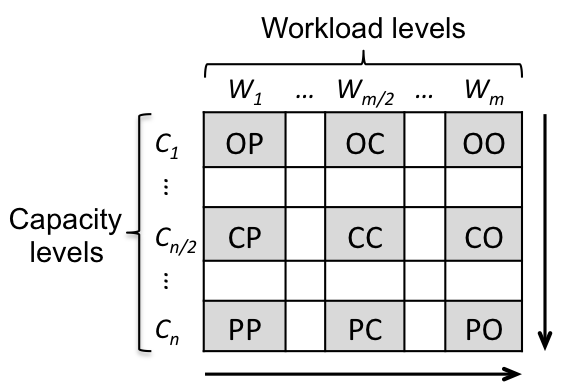
\includegraphics[scale=.8]{img/heuristics}
  \end{center}
  \caption{\label{fig:heuristicas}Ilustração das estratégias de seleção de Configurações e Cargas de Trabalho utilizadas pelas 9 Heurísticas de Seleção.}
\end{figure}

A imagem ilustra dois conjuntos dispostos em forma de matriz, um conjunto 
na vertical, formando as linhas, composto de $n$ Configurações $C_1 \ldots C_{n/2} 
\ldots C_n$ e um conjunto composto de $m$ Cargas de Trabalho $W_1 \ldots W_{m/2} 
\ldots W_m$, formando as colunas. As células dessa matriz mostram as Heurísticas
que selecionariam o par formado pela Configuração e pela Carga de Trabalho referentes
à linha e coluna da célula. Nessa representação das Heurísticas, a primeira letra
refere-se à abordagem usada para a escolha da Configuração e a segunda letra refere-se 
à abordagem usada na escolha da Carga de Trabalho.
 
Podemos ver, então, que as Heurísticas com abordagem Otimista escolherão Configurações 
mais próximas a $C_1$ e Cargas de Trabalho mais próximas a $W_m$. Por serem otimistas, essas 
abordagens consideram que máquinas menores são capazes de executar a aplicação com o nível esperado de desempenho sob cargas 
mais severas.

Ainda com base na mesma imagem, vemos que as abordagens conservadoras se concentram
nas células intermediárias, conforme a descrição das Heurísticas. A Heurística
OC, otimista para Configurações e conservadora para Cargas, se concentra na 
primeira linha, ou seja, mais próxima de $C_1$, e nas colunas do centro, mais
próximas de $W_{n/2}$. Observação similar se faz para a Heurística PO, pessimista 
para Configurações e otimista para Cargas, concentrando-se nas últimas linhas e 
últimas colunas, ou seja, Configurações e Cargas maiores.

Voltando a tratar das Estratégias de Avaliação, estas serão responsáveis por efetuar
a escolha de Configurações e Cargas de Trabalho implementando a lógica prevista pelas
Heurísticas. Enquanto as Heurísticas são lógicas que indicam as proximidades onde 
deve ser feita a escolha de Configurações e Cargas, a Estratégia implementa de fato
um algoritmo que reflita o comportamento esperado pela ideia da Heurística.
 
A aplicação das Heurísticas de Seleção, através da implementação de Estratégias 
de Avaliação, está intrinsecamente ligada aos objetivos deste trabalho, que é estudar 
os efeitos da inferência de desempenho na eficiência do processo de avaliação de 
capacidade para aplicações em ambientes de nuvem IaaS. A inteligência 
das Heurísticas propostas, ou seja, sua capacidade de escolher corretamente as 
Configurações e Cargas de Trabalho, é determinante para o sucesso do processo e 
da técnica de inferência. A eficácia e efetividade da aplicação das heurísticas
é analisada no Capítulo~\ref{chap:resultados}. 

\subsection{Funcionamento do Processo}
\label{sec:funcionamento_processo}
Para efeito de entendimento do funcionamento geral do processo de avaliação de 
capacidade ora proposto, podemos abstrair temporariamente o comportamento das 
Heurísticas. Esta é, aliás, outra vantagem da abordagem adotada de 
delegação de funções específicas a atividades customizadas: além da flexibilidade e 
adaptabilidade, a abstração dessas operações torna mais fácil o entendimento, 
a descrição e a implementação concreta do processo.

\begin{figure}
  \begin{center}
    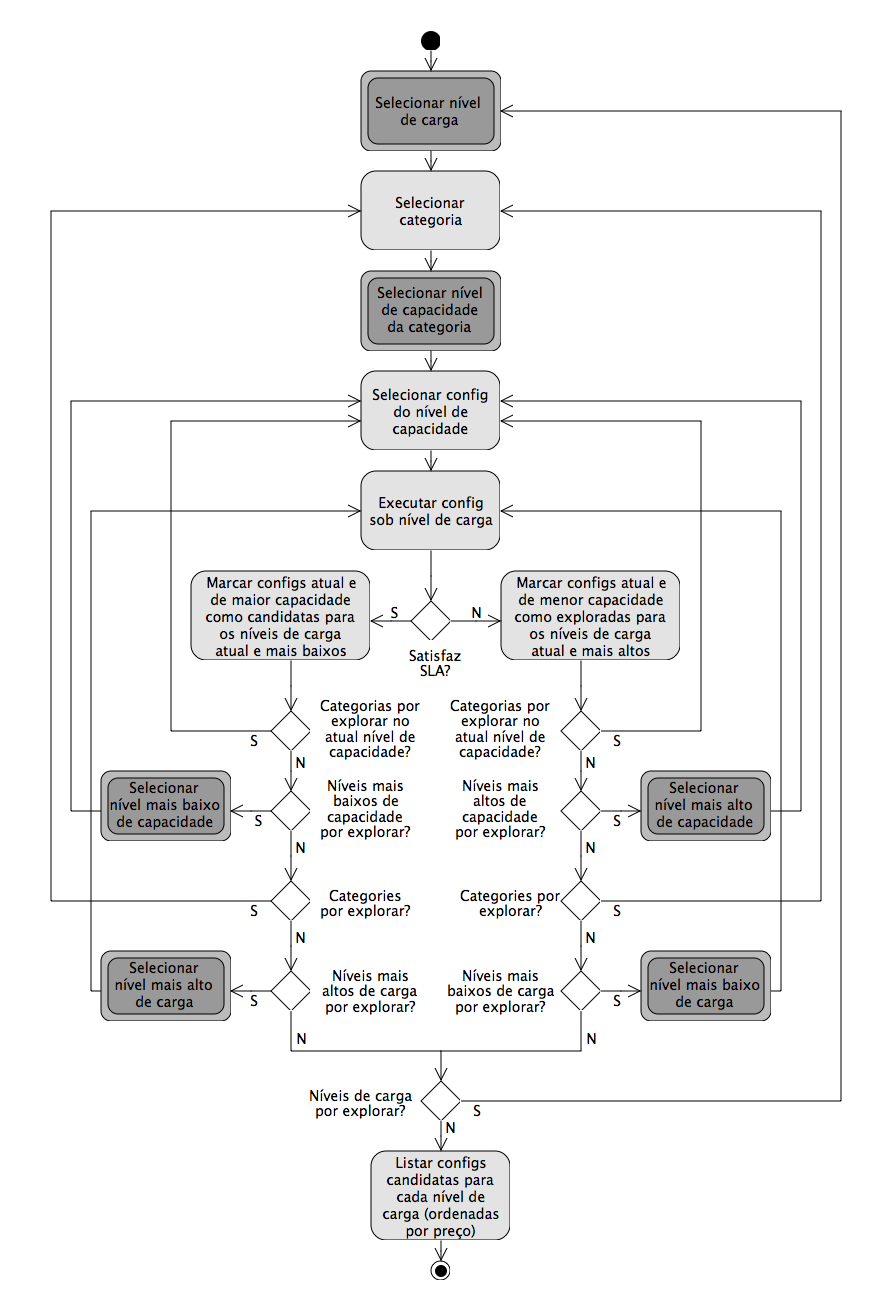
\includegraphics[scale=0.5]{img/capacity-planning-diagram-v13-mono}
  \end{center}
  \caption{\label{fig:fig_processo_aval_capacidade}Diagrama de atividades do Processo de Avaliação de Capacidade.}
\end{figure}


No diagrama de atividades representado na Figura~\ref{fig:fig_processo_aval_capacidade}, os blocos em destaque representam as operações que o processo espera que sejam executadas por uma Estratégia de 
Avaliação que implemente alguma das Heurísticas propostas na seção anterior. Os outros 
blocos referem-se a ações comuns do próprio processo, executadas de maneira 
idêntica independentemente de qual seja a Aplicação sob Teste ou de qual seja a 
Estratégia de Avaliação usada. A delegação de funções para a atividade de Execução
de Testes não está destacada no diagrama e se dá no passo ``\emph{Executar
config sob nível de carga}'', situado aproximadamente no centro da figura.

\subsubsection{Operações iniciais}
\label{subsec:processo_operacoes_iniciais}
Uma vez tendo recebido os dados de entrada, o Processo tem seu início com o momento 
de escolher por onde começar a execução dos testes.

A primeira atividade desempenhada pelo Processo é a escolha da Carga de Trabalho
inicial. A Estratégia é solicitada para realizar esta escolha, que deve
seguir a orientação dada pela lógica da Heurística selecionada para 
a avaliação. Assim, será escolhido
um volume de carga maior se a Heurística for Otimista, um volume menor se a
Heurística for Pessimista, ou um volume intermediário se a Heurística for Conservadora. 

Depois de selecionar o nível de carga, o processo segue para selecionar a
Categoria. Conforme as definições apresentadas na Seção~\ref{subsec:definicoes_categorias}, 
os Tipos de Máquinas Virtuais oferecidos pelo Provedor são normalmente agrupados 
por Categorias, que reunem máquinas de propósito e atributos semelhantes. Dessa
forma, o Espaço de Implantação sobre o qual a avaliação de capacidade se dará está 
dividido em Categorias. O número de Categorias envolvidas na avaliação depende do 
conjunto de Tipos de Máquinas Virtuais selecionados pelo usuário e passados como
parte dos dados de entrada do Processo.

O Processo de Avaliação seleciona a primeira
Categoria de máquinas a ser explorada. O processo não especifica a ordem ou método 
dessa escolha, pois essa ordem não é importante uma vez que todas as Categorias 
presentes no Espaço de Implantação serão avaliadas. Conforme veremos no 
Capítulo~\ref{chap:capacitor}, a implementação de referência do Processo 
desenvolvida neste trabalho escolhe a primeira Categoria em ordem alfabética pelo
nome. Outras implementações do processo podem optar por outros métodos de
escolha.



\paragraph{Níveis de Capacidade}
\label{subsec:processo_niveis_capacidade}
Dando continuidade à sequência de operações iniciais dentro do Processo de Avaliação 
de Capacidade, o próximo passo prevê que a Estratégia de Avaliação deve selecionar 
um Nível de Capacidade inicial. 

Níveis de Capacidade são um conceito criado para ajudar a estabelecer uma hierarquia 
sobre as relações de capacidade de processamento entre as diversas Configurações. 
Essa hierarquia de capacidade é válida apenas entre Configurações de uma mesma 
Categoria de Máquinas Virtuais. 

Para cada Categoria, o Nível ``um'' de Capacidade é composto apenas pela Configuração 
de menor preço dentro da Categoria. Um novo nível é criado com todas as Configurações 
para as quais é verdadeira a relação ``maior que''. Considera-se que uma 
Configuração $C_1$ é ``maior que'' uma outra Configuração $C_2$ se: 

\begin{enumerate}%[label=\bfseries \alph*)]
\item ambas são formadas pelo mesmo Tipo de Máquina Virtual e $C_1$ possui 
número maior de instâncias do que $C_2$; ou
\item ambas são formadas pelo mesmo número de instâncias
e o Tipo de Máquina de $C_1$ possui mais CPU e mais memória que o Tipo de Máquina
de $C_2$.  
\end{enumerate}

Esse, então, passa a ser o Nível 
``dois'' e a lógica se repete daí em diante, tomando-se, para cada Configuração 
desse nível, as imediatamente maiores, formando um novo Nível. O procedimento 
continua até que todas as Configurações estejam devidamente classificadas em 
Níveis de Capacidade.

A Figura~\ref{fig_niveis_capacidade} mostra um pequeno exemplo, onde 6 Configurações,
pertencentes a duas Categorias distintas, foram classificadas em dois Níveis de 
Capacidade dentro de cada Categoria. Os retângulos representam as Configurações, 
com o texto indicando o nome do Tipo de Máquina Virtual utilizado e o número entre 
parênteses representando a quantidade de instâncias que compõem a Configuração. 
As setas que ligam as Configurações indicam a existência da relação de capacidade 
entre elas apontando da menor para a maior. A ausência de seta entre duas Configurações 
implica a impossibilidade de se afirmar uma relação de capacidade entre elas. 

\begin{figure}[t]
  \begin{center}
    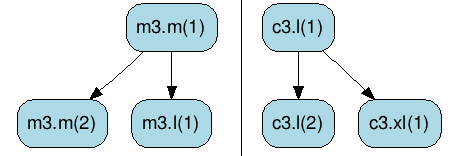
\includegraphics[scale=.65]{img/exemplo-niveis-capacidade}
  \end{center}
  \caption{\label{fig_niveis_capacidade}Agrupamento de Configurações por Níveis de Capacidade}
\end{figure}

Assim, observando o Espaço de Implantação organizado por Categorias e classificado
hierarquicamente, a Estratégia deve selecionar, com base em uma das Heurísticas 
propostas na subseção anterior, um Nível de Capacidade inicial. As 
Configurações que fazem parte do Nível inicial escolhido são disponibilizadas 
para que a Avaliação proceda com a execução dos testes da Aplicação.

\subsubsection{Execução do Teste de Desempenho}
\label{subsec:processo_execucao}
Após a escolha da Carga de Trabalho inicial e do primeiro Nível de Capacidade a
ser avaliado, uma Configuração deve ser tomada a partir do Nível de Capacidade 
atual. Essa seleção não segue nenhuma regra específica, uma vez que todas as 
Configurações do Nível de Capacidade devem ser avaliados, ainda que por meio da técnica de 
Inferência de Desempenho, vista adiante.
 
Executa-se, então, a Aplicação sob Teste, impondo-se a ela a Carga de Trabalho 
selecionada, e analisa-se o resultado dessa execução. Nesse ponto o Processo se 
bifurca, atingindo seu primeiro ponto de decisão.

Esse é o momento em que a técnica de Inferência, conforme propomos neste trabalho,
será aplicada. A análise do Resultado obtido, mais especificamente do valor atribuído
à Métrica de Desempenho avaliada, comparado ao parâmetro do Valor de Referência (SLA), 
determina se a Aplicação é ou não capaz de atender à demanda imposta pela
Carga de Trabalho. Vejamos a seguir uma explanação mais detalhada a respeito das
inferências que sucedem essa análise.  

\subsubsection{Inferência de Desempenho}
O processo de Inferência de Desempenho acontece logo após a análise comparativa
do Resultado, conseguinte a uma execução real da Aplicação sob Teste em uma 
Configuração, que foi tomada a partir de um Nível de Capacidade previamente 
selecionado. Durante essa execução, foi imposta sobre a Aplicação uma Carga de 
Trabalho, também previamente selecionada.

Observando o diagrama da Figura~\ref{fig:fig_processo_aval_capacidade}, podemos 
ver, bem ao centro, o ponto de decisão que define o sucesso ou o fracasso da 
Aplicação em atingir o SLA exigido. 

Se o desempenho da Aplicação satisfaz o SLA proposto, o Processo considera que a
Configuração é capaz de executar sob a Carga de Trabalho imposta e diz que a 
Configuração atual (sobre a qual a Aplicação acabou de ser executada) deve ser
assinalada como uma Configuração Candidata.

Neste ponto, a técnica de Inferência de Desempenho é aplicada e, como vemos
no texto do diagrama do Processo, todas as Configurações maiores que a atual também
são assinaladas como Candidatas. Ora, se identificamos que uma certa Configuração
consegue executar a Aplicação sob uma certa Carga de Trabalho, é intuitivo o 
pensamento de que qualquer Configuração que possua maior poder computacional 
também seja capaz de executar a mesma Aplicação sob a mesma Carga de Trabalho.

Assim, usando a representação do Espaço de Implantação conforme descrito na
Seção~\ref{subsec:processo_niveis_capacidade}, o Processo assinala como candidatas
todas as Configurações para as quais, direta ou indiretamente, a Configuração 
atual aponte, ou seja, todas as Configurações que, de acordo com o grafo de capacidade representado no Espaço de Implantação, seriam ``maiores que'' a Configuração atual. 

Mas a técnica de Inferência ainda vai mais longe. Sabendo que as Configurações
que acabaram de ser assinaladas como Candidatas são capazes de executar a Aplicação
sob a Carga de Trabalho atual, também é intuitivo concluir que Cargas de Trabalho 
menores, ou mais brandas, serão naturalmente atendidas por essas mesmas Configurações.

Então, com base na Inferência de Desempenho, o Processo marca
a Configuração atual e todas as maiores que ela como Candidatas não só para a 
Carga de Trabalho atual, mas também para todas as Cargas inferiores à atual.

De volta ao ponto de decisão da análise do Resultado em relação ao SLA, caso o 
desempenho da Aplicação não satisfaça o SLA, o Processo considera que a 
Configuração não é capaz de executar sob a Carga de Trabalho atual. Assim, essa
Configuração é marcada como Rejeitada para tal Carga.

De forma coerente, a lógica de Inferência de Desempenho entende que, se dada 
Configuração não consegue executar uma Aplicação a contento sob uma certa Carga,
intuitivamente, as Configurações menores tampouco conseguirão. Assim, o processo
indica a marcação de todas as Configurações ``menores que'' a atual como 
Rejeitadas para a Carga de Trabalho atual. 

Ainda seguindo a Inferência de Desempenho, quando uma Configuração não consegue
atender a demanda de uma Carga de Trabalho, presume-se que também não consiga
atender a demandas maiores, ou mais severas. O Processo de Avaliação marca, então,
a Configuração atual e todas as Configurações menores que ela como Rejeitadas para todas as Cargas de Trabalho maiores que a Carga atual. 

\begin{figure}[t]
  \begin{center}
    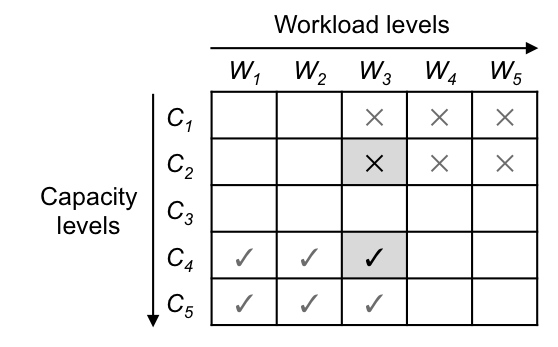
\includegraphics[scale=.8]{img/inference}
  \end{center}
  \caption{\label{fig:fig_processo_inferencia}Ilustração da marcação de Configurações Candidatas (à esquerda) e Rejeitadas (à direita) com a técnica de Inferência de Desempenho.}
\end{figure}

O efeito da utilização da técnica de Inferência de Desempenho pode ser melhor
visualizado através dos exemplos mostrados na Figura~\ref{fig:fig_processo_inferencia}. A figura mostra 
duas situações: a da esquerda para o caso em que o SLA é satisfeito e a da direita 
caso o SLA não seja satisfeito. Em ambos os casos vemos uma célula central realçada, 
indicando que a Aplicação sob Teste foi executada na Configuração $C_3$ sob a 
Carga de Trabalho $W_3$. As células assinaladas com com um ``\boldmath$\surd{}$'' mostram as Configurações
marcadas como Candidatas para as Cargas de Trabalho correspondentes. As células
assinaladas com um ``\boldmath$\times{}$'' representam as Configurações marcadas como Rejeitadas.

Essa representação serve para demonstrar a contribuição da utilização da técnica 
de Inferência na execução de testes de desempenho. Nesse exemplo, foram 
explorados 9 cenários diferentes, dados pelas combinações de Configurações e 
Cargas de Trabalho, mas apenas 1 execução real foi conduzida. Isso significa não
só que o tempo total gasto na Avaliação de Capacidade é reduzido, mas também o
custo financeiro envolvido nessa atividade. 

Mais adiante neste capítulo, expandiremos essa representação para mostrar a ação
da Inferência de Desempenho após várias iterações do laço compreendido pelo 
Processo de Avaliação. Por hora, continuemos com a descrição dos passos seguintes.

\subsubsection{Seleção dos Próximos Cenários}
\label{subsec:selecao_cenarios}
Passada a fase de Inferência de Desempenho, o processo segue seu caminho, tomando
as decisões que levarão à seleção dos cenários seguintes a serem avaliados quanto
à sua capacidade.

O ponto de decisão que sucede a marcação das Configurações Candidatas ou Rejeitadas
checa se existem Configurações pertencentes ao atual Nível de Capacidade cujas 
execuções ainda não tenham sido avaliadas para a Carga de Trabalho atual. Se 
existirem, o Processo volta ao passo de seleção de uma Configuração a partir do 
Nível de Capacidade e uma nova execução é solicitada.

Se não existirem Configurações inexploradas para a Carga de Trabalho atual no
Nível de Capacidade corrente, o Processo buscará por um Nível de Capacidade que 
ainda não tenha sido completamente explorado. Se a Aplicação satisfez o SLA na 
execução anterior, a Estratégia deverá selecionar um Nível de Capacidade menor. 
Se o SLA não tiver sido atingido, a Estratégia tentará selecionar um  Nível de 
Capacidade maior. Depois de selecionado o próximo Nível de Capacidade, o laço do
Processo retorna ao ponto de seleção da próxima Configuração e outra execução 
acontece.
   
Novo ponto de decisão surge quando a Estratégia não encontra um Nível de 
Capacidade a ser explorado. Nessa situação, o Processo procura uma outra
Categoria dentro do Espaço de Implantação que ainda possua pelo menos uma
Configuração ainda não explorada para a Carga de Trabalho atual. Se houver,
o Processo retorna ao passo de seleção de um Nível de Capacidade dentro da
Categoria selecionada e nova execução será realizada.

Caso não haja uma outra Categoria com Configurações não avaliadas, atingimos
então um outro ponto de decisão, onde a Estratégia deve buscar uma Carga 
de Trabalho que não tenha sido avaliada. Se a execução anterior atingiu o SLA,
uma Carga de Trabalho maior será buscada. Caso contrário, a Estratégia tentará
uma Carga menor que a atualmente selecionada. Se a Estratégia obtiver sucesso
nessa escolha, o Processo dispara uma nova execução da Aplicação com a Configuração
corrente e sob a Carga de Trabalho que acabou de ser selecionada.

Porém, se a Estratégia não conseguir fornecer uma Carga de Trabalho segundo as 
restrições do Processo definidas a partir da comparação do Resultado com o SLA, o Processo 
voltará ao passo inicial de seleção de Carga de Trabalho, que não tem qualquer 
restrição quanto a essa seleção. Tentará assim a escolha de uma Carga inexplorada
qualquer. Caso não seja encontrada nenhuma Carga de Trabalho inexplorada, significa
que não há mais nada a ser testado e o Processo é encerrado.

\subsubsection{Finalização da Avaliação}
Não tendo mais Configurações a serem testadas sob nenhuma Carga de Trabalho, o 
Processo é dado por concluído e sua finalização se efetiva pela apresentação de uma
lista que contém, para cada Carga de Trabalho, as Configurações capazes de executar
a Aplicação sob Teste, em ordem crescente de preço.

Por ``capazes de executar'', entenda-se como as Configurações para as quais o valor
obtido para a Métrica de Desempenho durante a execução da Aplicação sob determinada
Carga de Trabalho é menor ou igual ao valor definido para o SLA
como parte dos dados de entrada do Processo.

Embora essa seja a resposta final do processo, a contribuição real deste trabalho está
na maneira como chegamos a essa resposta, com redução de custo e tempo, e na precisão 
da resposta, ou seja, o nível de acerto atingido pelo Processo ao apontar as Configurações
Candidatas e Rejeitadas. Dados reais que comprovam a eficácia do 
Processo e da técnica de Inferência de Desempenho propostos são apresentados no
Capítulo~\ref{chap:resultados}, que trata dos experimentos realizados e analisa criticamente os resultados obtidos.

Para deixar mais clara essa contribuição, a seguir é dado um exemplo que ilustra os vários momentos
em que a técnica de Inferência de Desempenho é empregada durante a execução do Processo, e que evidencia a influência que a utilização de diferentes Heurísticas de Seleção exerce sobre a sua eficiência em selecionar as melhores configurações de recursos para a aplicação alvo.

...



\subsection{Exemplo de Uso}

\subsection{Implementação}

\section{Avaliação Experimental}\label{sec:experiments}

\subsection{Metodologia}

\subsection{Resultados}

\subsubsection{Acurácia}

\subsubsection{Eficiência}

\section{Trabalhos Relacionados}\label{sec:related-work}

Os trabalhos que apoiam os usuários de nuvens IaaS no planejamento de capacidade
das suas aplicações fazem uso de uma abordagem preditiva ou de uma abordagem
empírica para propor a configuração mais adequada para a aplicação. Na abordagem
preditiva, os trabalhos não executam diretamente a aplicação alvo no ambiente
onde se deseja
implantá-la,~\cite{cloudharmony},~\cite{malkowski2010cloudxplor,li2011,jung2013cloudadvisor,fittkau2012cdosim} e~\cite{li2011cloudprophet}.
Já na abordagem empírica, as aplicações alvo são implantadas na
nuvem e então submetidas a testes de
carga,~\cite{jayasinghe2012,silva2013cloudbench,cunhacloud}
e~\cite{scheuner2014cloud}.

As soluções de abordagem preditiva não requerem a alocação de
recursos de nuvem para realizarem as predições, com
exceção do \textit{CloudProphet}, apresentado em~\cite{li2011cloudprophet}, que
requer a alocação de recursos da nuvem para avaliar todas as demandas e configurações.
Além disso, são soluções de baixa complexidade, com destaque para a
apresentada em \cite{cloudharmony}, a qual permite que os testes sejam
iniciados e que as pesquisas de resultados anteriores sejam realizadas através de uma
interface amigável, sem a necessidade de intervenções do usuário. Por outro
lado, essas soluções apresentam limitações na definição da aplicação alvo e
seus requisitos de desempenho,~\cite{malkowski2010cloudxplor,cloudharmony}, e os
resultados das predições podem divergir dos valores reais. O que
ficou evidenciado em~\cite{fittkau2012cdosim} cujos resultados de algumas
simulações mostraram que a taxa de error da utilização de CPU simulada com a
utilização de CPU medida, chegou a 30,86~\%. 

Por sua vez, o \textit{CloudProphet} apresentando em~\cite{li2011cloudprophet},
é uma solução de abordagem preditiva que permite ao usuário definir aplicação,
demanda, recurso da nuvem e SLA desejado, o que também é permitido pelas
soluções de abordagem empírica. Por exemplo, na solução apresentada
em~\cite{cunhacloud}, o usuário pode definir toda a pilha de componentes
da aplicação alvo, todos cenários utilizados na avaliação de desempenho, as
demandas que serão submetidas a cada um dos cenários e o critério que define se
o cenário suportou a demanda, ou seja, o SLA. Da mesma forma, as soluções
apresentadas em~\cite{jayasinghe2012,silva2013cloudbench,scheuner2014cloud},
possuem os seus mecanismos para a realização dessas definições.

Apesar das soluções de abordagem empírica oferecerem grande liberdade na
definição das aplicações, elas precisam executar cada um dos cenários definidos
pelo usuário e não fazem uso de resultados anteriores para evitar a
execução de testes que claramente poderiam ser evitados. Por exemplo, em uma
situação na qual uma demanda é submetida à aplicação que está sendo executada em
uma máquina virtual com baixo poder computacional, seria coerente afirmar que
essa mesma demanda pode ser atendida por máquinas com perfis computacionais mais
robustos. Já no que diz respeito à complexidade, cada trabalho faz uso de uma
estratégia de uso particular. Dessa forma, as experiências anteriores do usuário
irão ser determinantes na percepção da complexidade. Pois esse usuário precisa
se adaptar à sintaxe de cada solução, e eventualmente, configurar imagens
contendo os componentes da aplicação que será avaliada.

\section{Conclusão}\label{sec:conclusion}


\section*{Agradecimentos}
Este trabalho é parcialmente financiado pelo Conselho Nacional de Desenvolvimento Científico e Tecnológico (CNPq), através dos processos 311617/2011-5 e 487174/2012-7.

\bibliographystyle{sbc}
\bibliography{principal}
\end{document}